\chapter{Implementierung} \label{sec:Implementierung}
\section{Versionsverwaltung mit Subversion} \label{sec:impl-Versionsverwaltung}
Als Versionsverwaltung wurde Subversion verwendet. Dies hat mehrere Gr�nde: Zum einen war Subversion zu diesem Zeitpunkt eine neue und z.T. auch unbekannte Technologie, die somit ihren Reiz hatte. Zum anderen wurde Subversion als Nachfolger von CVS angepriesen und sollte viele Nachteile eliminieren. Eins der wichtigen Vorteile von Subversion ist die geringe Netzwerklast. Bei einem "`Commit"' werden nur die Unterschiede zur Vorg�ngerversion �bertragen und nicht wie bei CVS jede Datei komplett. Um Subversion verwenden zu k�nnen, wurde ein Rechner mit einem installieren Subversion Server ben�tigt, der m�glichst 24h im Internet verf�gbar ist. Um mit einem Client auf einen Subversion Server zuzugreifen, gibt es verschiedene �bertragungsprotokolle: Ein eigenes Subversion protokoll (svn), eine Kombination aus Secure Shell und dem eigenen Protokoll (ssh+svn), �ber http oder �ber https. Die sicherste Methode �ber ssh+svn, jedoch erfordert diese die Installation eines SSH Server, was unter Linux, dank verschiedener Anleitungen, einfach geht, jedoch unter Windows nicht so einfach zu realisieren ist. Unter Windows wurde zu Testzwecken ein Apache2 Webserver mit einem Zertifikat zur �bertragung von Daten per https installiert. Dieser Webserver wurde mit dem Subversion Server kombiniert und jeglicher Datentransfer f�r Subversion erfolgte �ber https und dessen eingestellen Port. Der Nachteil war jedoch, dass keiner die M�glichkeit hatte, einen PC 24h online zur Verf�gung zu stellen. So wurde nach einiger Suche im Internet der Open Source Anbieter Berlios Developer\footnote{\url{http://developer.berlios.de/}} entdeckt. Dort k�nnen Open-Source Projekte ihre Quellcodes in einer Subversion Versionsverwaltung mittels ssh+svn kostenlos speichern. Bei Berlios ist das Repository bereits erstellt, bei unseren Testsystem musste dies mit einem einfachen Befehl manuell erfolgen:
\begin{verbatim}
svnadmin create f:/subversion/phil/daten
\end{verbatim}
Durch diesen Befehl wurde in dem angegebenen Verzeichniss durch den Befehl \texttt{svadmin create} ein neues Repository erzeugt, das im Dateisystem auf dem Server die folgende Verzeichnissstruktur wie in \vref{fig:svnverzeichniss} zu sehen ist, besitzt.
\begin{figure}[htbp]
	\centering
	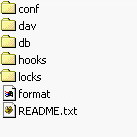
\includegraphics[scale=1.0]{images/svn-verzeichniss-struktur.jpg}
	\caption{Verzeichnissstruktur des Repository auf dem Server}
	\label{fig:svnverzeichniss}
\end{figure}
Im Verzeichniss \texttt{conf} befinden sich zwei wichtige Dateien. In der svnserve.conf, wie in \vref{code:svnserve} zu sehen, sind grundlegende Eigenschaften wie Zugangsberechntigungen, Begr��ung und Passwortdatei festgelegt. In der Passwortdatei, wie in \vref{code:svnuser} zu sehen, werden Benutzernamen und Passw�rter f�r die Benutzer dieses Repository vergeben. Diese Methode der Authentisierung ist jedoch nicht zu empfehlen, da die Passw�rter in diesen Dateien lesbar sind und diese Datei, zus�tzlich zu anderen bereits vorhandenen Zugangslisten, aktuell gehalten werden muss.
\begin{lstlisting}[language=Java, showstringspaces=false, caption={Datei /conf/svnserve.conf},label=code:svnserve]
[general]
anon-access = none
auth-access = write
realm = Repository for my personal diplomarbeit
password-db = user
\end{lstlisting}
\begin{lstlisting}[language=Java, showstringspaces=false, caption={/conf/user},label=code:svnuser]
[users]
pschneider = geheim
\end{lstlisting}
Eine bessere M�glichkeit der Authentisierung w�re die �berpr�fung, bevor der Benutzer Zugang zum System erh�lt. Bei einer ssh+svn erfolgt die Authensisierung durch ssh und bei https erfolgt diese �ber htaccess, in beiden F�llen wird dabei wahrscheinlich auf einen vorhandenen Authentisierungsinfrastruktur zur�ckgegriffen.\\
\begin{figure}[htbp]
	\centering
	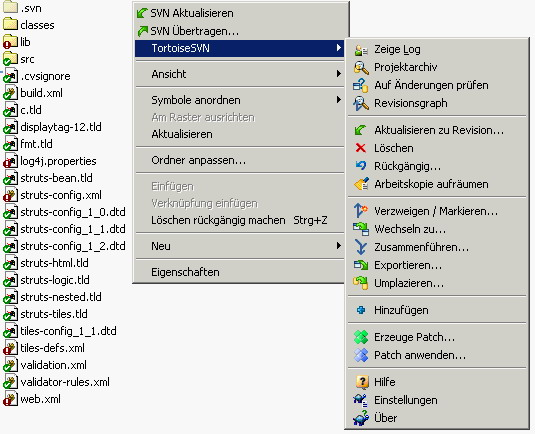
\includegraphics[scale=0.75]{images/svn-verzeichniss-client.jpg}
	\caption{Ansicht des Clients TortoiseSVN}
	\label{fig:svnclient}
\end{figure}
In unserem Projekt wurde als Client f�r den Zugriff auf das Subversionrepository TortoiseSvn\footnote{\url{http://tortoisesvn.tigris.org/}} verwendet. Dabei handelt es sich wie in \vref{fig:svnclient} zu sehen, um eine Windows-Shellerweiterung, die sich in den Explorer integriert. Ist ein Verzeichniss oder eine Datei Teil eines Projektes, das in einer Subversionversionsverwaltung gespeichert wird, sind diese durch kleine farbige Symbole markiert. Diese Symbole geben den Zustand der Dateien an, ob diese aktuell sind, ver�ndert wurde oder ob eventuelle Konflikte bestehen. Weiterhin k�nnen damit auch alle anderen Aktionen wie Log Datei betrachten, R�ckg�nging, Tagging/Merging und Verschiebungen wie in \vref{fig:svnclient} zu sehen, vorgenommen werden. Mit TortoiseSVN ist auch m�glich nur ein bestimmtes Verzeichnis des meist sehr strukturiertes Projektes auszuchecken und zu bearbeiten. Dazu wird 
\texttt{TortoiseSVN $\Rightarrow$ Wechseln zu }
wie in \vref{fig:svnwechselnzu} zu sehen ausgew�hlt. In dem sich �ffnenden Dialog wird das entsprechende Verzeichnis im Repository gew�hlt und die lokale Arbeitskopie wird automatisch auf die entsprechenden Verzeichnisse und Dateien aktualisiert.\\
\begin{figure}[htbp]
	\centering
	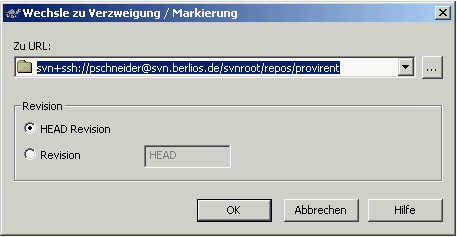
\includegraphics[scale=0.75]{images/svn-wechselnzu.jpg}
	\caption{Ansicht des Fensters zum wechseln der Arbeitskopie}
	\label{fig:svnwechselnzu}
\end{figure}
In den Einstellungen des Subversionservers k�nnen auch wie in \vref{tech-svn} bereits beschrieben, automatisch Email verschickt werden. Die in \vref{code:emailcommit} gezeigte Email soll verdeutlichen, welche Informationen mit diesem Mechanismus verschickt werden k�nnen. Im Betreff der Email befindet sich die neue Revisionnummer und das Verzeichnis in dem die �nderungen stattgefunden haben. Am Anfang der Email ist der Name des Authors, das Datum, eine Auflistung der ge�nderten Dateien und die Logmeldung zu sehen. Am Ende befinden sich die kompletten �nderungen als Text.


\begin{lstlisting}[language=Java, showstringspaces=false, caption={Auszug aus einer automatisch erzeugten Email},label=code:emailcommit]
Author: rgriesch
Date: 2005-12-02 21:04:22 +0100 (Fri, 02 Dec 2005)
New Revision: 276

Modified:
   project_src/provirent_hibernate/src/de/hsharz/provirent/management/gui/ManagementGui.java
Log:
Menu Rechnung fehlt  - sollte aber aus Zeitgr?\195?\188nden                                nicht mehr implementiert                                   werden !!
ManagementGui        - Reiter Film war aktiv, obwohl
                       Fenster kunden angezeigt wurde
                       ( Fehler behoben )
ManagementGui        - Button Beenden im Menu "Datei"
                       wurde Funktionalit?\195?\164t eingef?\195?\188gt   

Modified: project_src/provirent_hibernate/src/de/hsharz/provirent/management/gui/ManagementGui.java
===================================================================
--- project_src/provirent_hibernate/src/de/hsharz/provirent/management/gui/ManagementGui.java	2005-11-30 15:04:55 UTC (rev 275)
+++ project_src/provirent_hibernate/src/de/hsharz/provirent/management/gui/ManagementGui.java	2005-12-02 20:04:22 UTC (rev 276)
@@ -412,9 +412,12 @@
 
 		exitMenuItem = new MenuItem(fileMenu, SWT.CASCADE);
 		exitMenuItem.setText(l.getString("menu.file.exit"));
-
+		exitMenuItem.addSelectionListener(new SelectionAdapter() {
+			public void widgetSelected(SelectionEvent evt) {
+			    shell.close();
+			}
+		});
 	}
-
 	/**
 	 * init the View Menu
 	 */
@@ -484,7 +487,7 @@
 
 		viewCustomerMenuItem = new MenuItem(viewMenu, SWT.CHECK);
 		viewCustomerMenuItem.setText(l.getString("menu.view.customer"));
-		viewCustomerMenuItem.setSelection(false);
+		viewCustomerMenuItem.setSelection(true);
 		viewCustomerMenuItem.addSelectionListener(new SelectionAdapter() {
 			public void widgetSelected(SelectionEvent evt) {
 				if (tabItemCustomer == null || tabItemCustomer.isDisposed()) {
@@ -599,7 +602,7 @@
 
 		viewMovieMenuItem = new MenuItem(viewMenu, SWT.CHECK);
 		viewMovieMenuItem.setText(l.getString("menu.view.movie"));
-		viewMovieMenuItem.setSelection(true);
+		viewMovieMenuItem.setSelection(false);
 		viewMovieMenuItem.addSelectionListener(new SelectionAdapter() {
 			public void widgetSelected(SelectionEvent evt) {
 				if (tabItemMovie == null || tabItemMovie.isDisposed()) {

_______________________________________________
Provirent-svn-commit mailing list
Provirent-svn-commit@lists.berlios.de
http://lists.berlios.de/mailman/listinfo/provirent-svn-commit
\end{lstlisting}















%Hier danach nicht mehr schreiben
\label{sec:impl-Versionsverwaltung-ende}
